\chapter{Proposed System and Methodology}
\label{ch:methodology}

\section{Proposed System Overview}

The system we built has three controllers that can each, one at a time, take
charge of scaling a single Kubernetes Deployment: a PPO reinforcement
learning agent, an HPA configured against CPU and memory utilization (our
resource baseline), and an HPA configured against CPU utilization only
(matching the pattern most Kubernetes deployments use out of the box, our
CPU baseline). All three act on the same Deployment, in the same namespace,
on the same Minikube cluster, and are never allowed to be active at the same
time -- a controller-exclusivity lock enforces this at acquisition time, so
that a run under one arm can never be contaminated by another controller's
decisions. A traffic generator drives load against the Deployment through a
benchmark FastAPI service; Prometheus scrapes telemetry from that service
and from the cluster; an evaluation/training harness orchestrates episodes,
tears down and restores canonical idle state between them, and records
every attempt, successful or not, to an append-only ledger.

\section{System Architecture}

Figure~\ref{fig:system-architecture} shows the full architecture. The
Minikube cluster hosts the benchmark application's pods, a Service in front
of them, the HPA object (when an HPA arm is active), the Metrics Server, and
Prometheus. A host-side load generator and relay process issues HTTP
requests against the cluster's exposed route, following a deterministic,
seeded schedule for the traffic profile currently in play. When the PPO arm
is active, a host-side agent process reads Prometheus and Kubernetes API
state, builds the eleven-feature observation described in
Section~\ref{sec:mdp}, runs it through the trained policy, passes the raw
action through the safety layer described in Section~\ref{sec:safety-layer},
and issues a \texttt{kubectl scale}-equivalent call against the Deployment.
The controller-exclusivity lock file ensures that, whichever arm is active,
it is the only process touching the Deployment's replica count.

\begin{figure}[htbp]
\centering
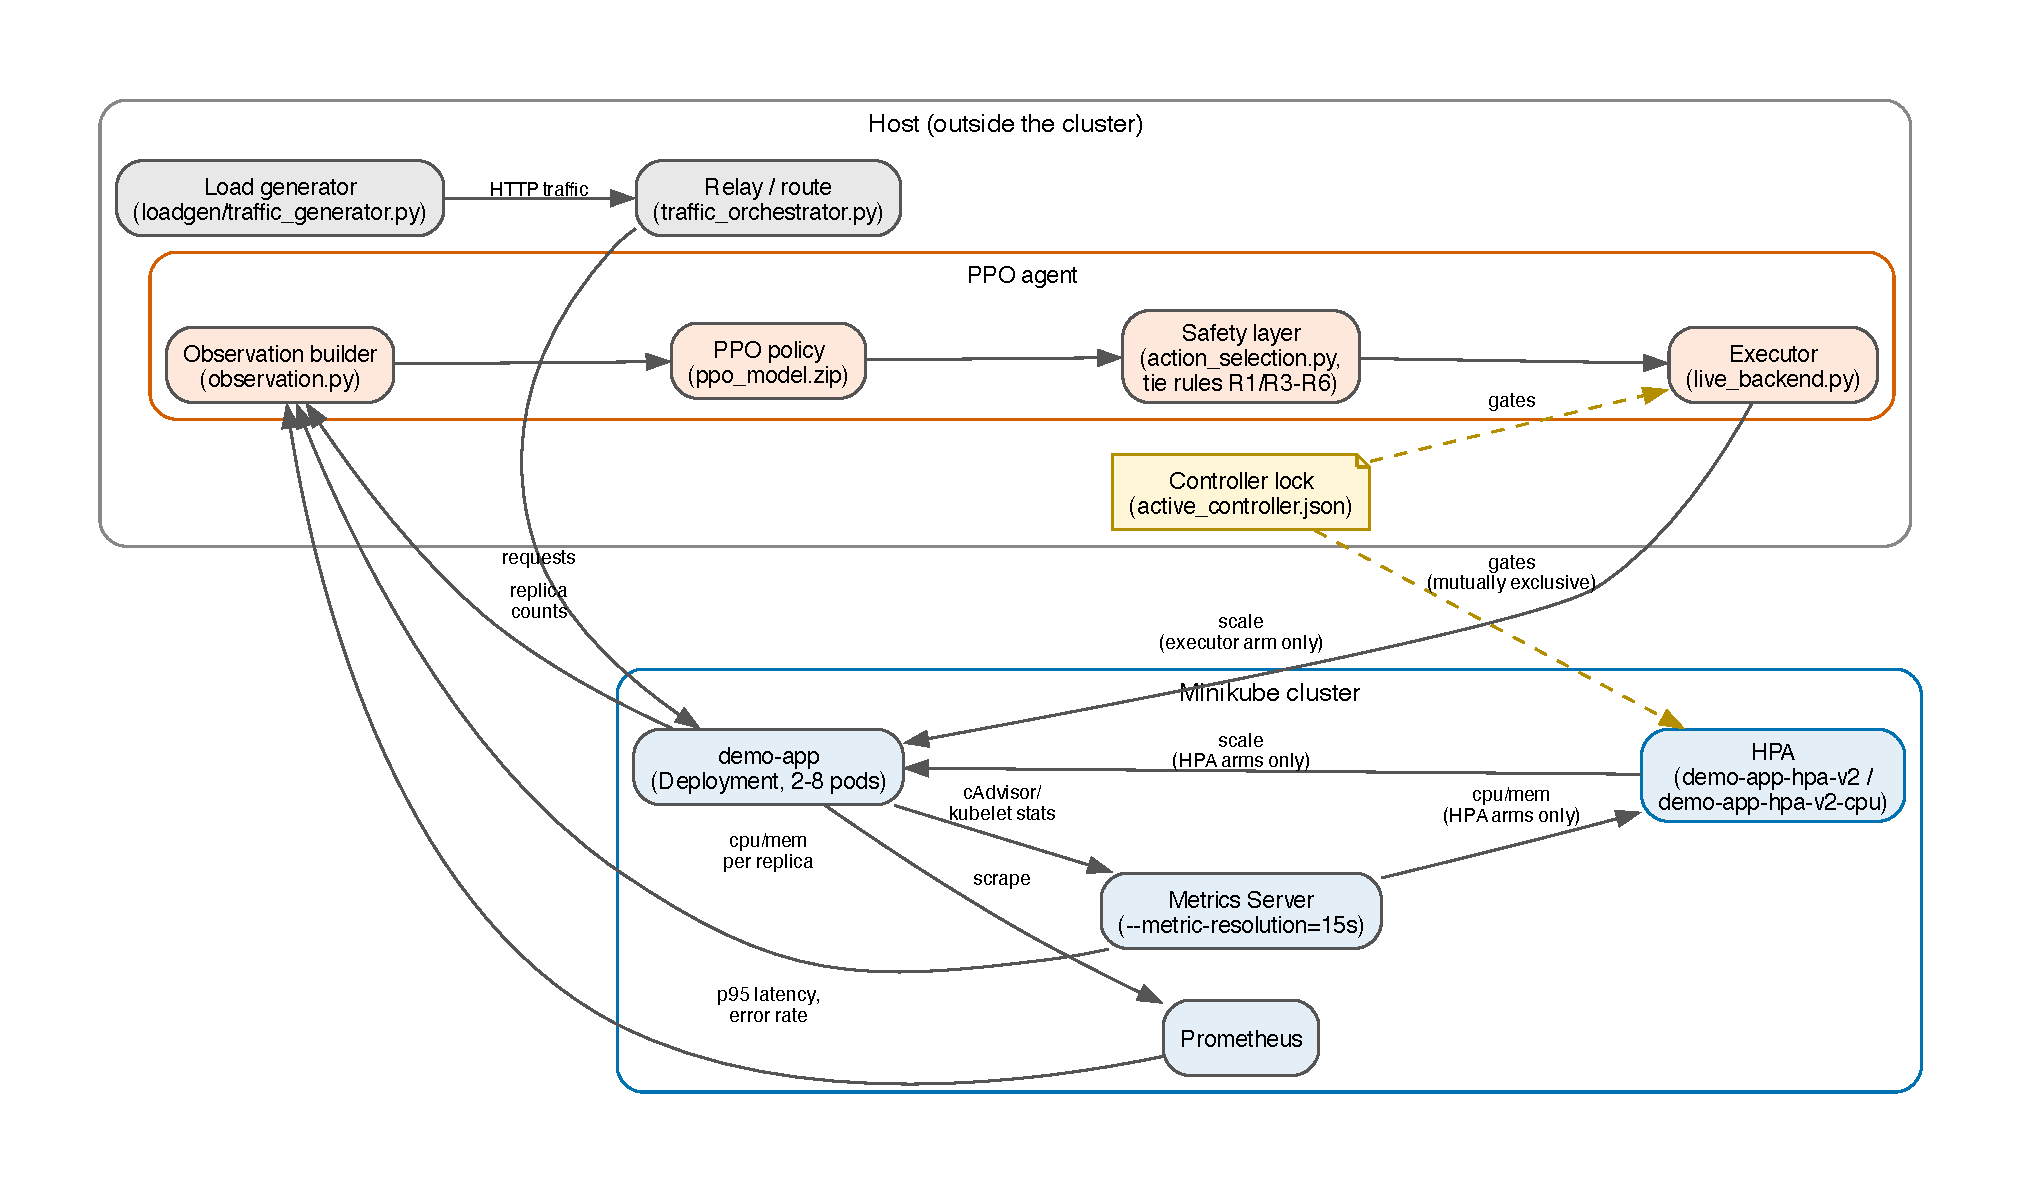
\includegraphics[width=0.95\textwidth]{../figures/diagram_system_architecture.pdf}
\caption{System architecture: the Minikube cluster (demo-app pods, HPA,
Metrics Server at a 15-second resolution, Prometheus) together with the
host-side load generator/relay and the PPO agent's
observation-builder\,$\rightarrow$\,policy\,$\rightarrow$\,safety-layer\,$\rightarrow$\,executor
pipeline, gated by a controller-exclusivity lock so that the PPO agent and
either HPA arm are never both active on the same Deployment at once.}
\label{fig:system-architecture}
\end{figure}

Figure~\ref{fig:rl-control-loop} shows the RL decision loop in isolation:
one 30-second cycle from observation to policy to safety gating to the
Kubernetes API to the resulting metrics to the reward computed from them,
feeding into the next PPO update.

\begin{figure}[htbp]
\centering
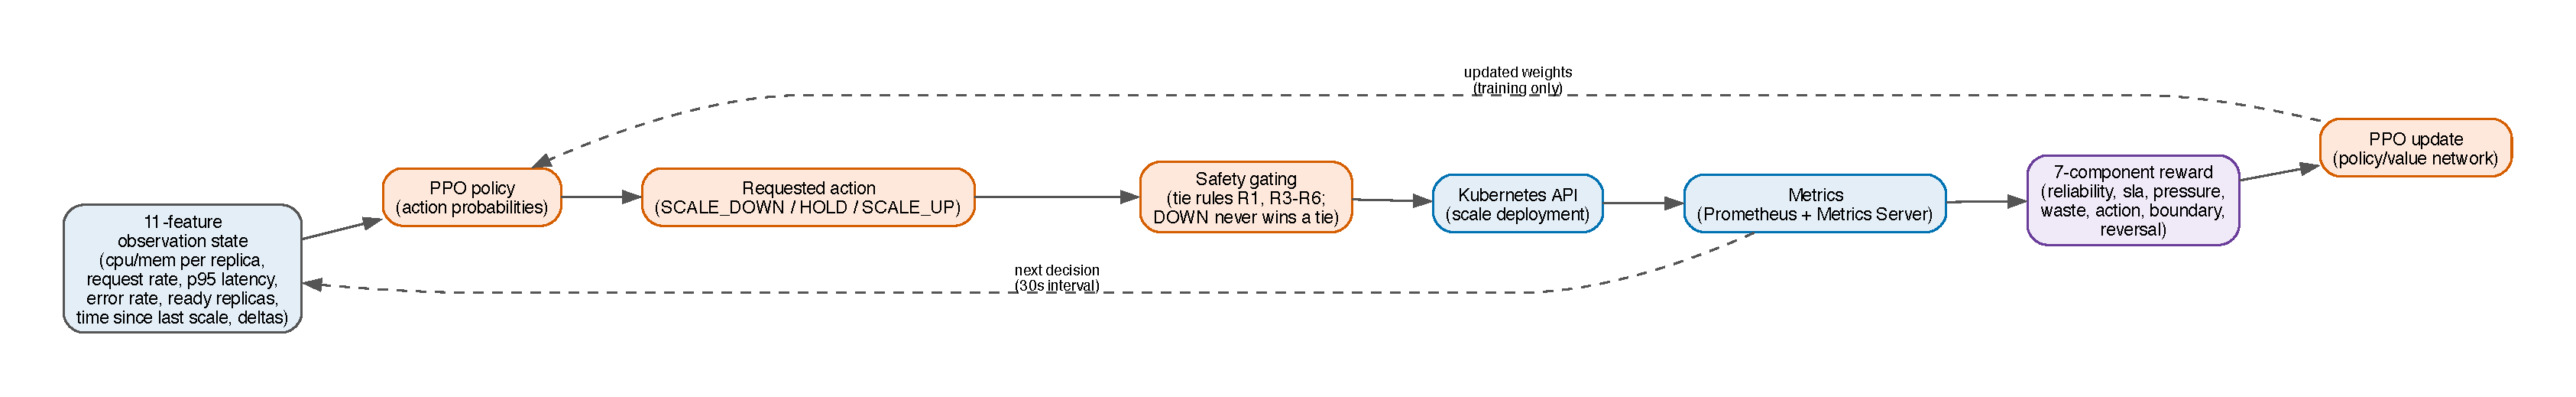
\includegraphics[width=0.85\textwidth]{../figures/diagram_rl_control_loop.pdf}
\caption{The RL control loop: the 11-feature observation feeds the PPO
policy, whose action passes through safety gating before reaching the
Kubernetes API; the resulting metrics feed the 7-component reward, which
feeds the next PPO update. One cycle corresponds to one 30-second decision
interval.}
\label{fig:rl-control-loop}
\end{figure}

Figure~\ref{fig:experiment-pipeline} places the whole project on a single
timeline: the V1 design, its evaluation and failure analysis, the V2
redesign, the 48-session V2 training campaign, the pre-registered V2
evaluation (\texttt{eval\_\allowbreak final}), and the later, separately labelled
exploratory stress test (\texttt{stress\_\allowbreak explore}).

\begin{figure}[htbp]
\centering
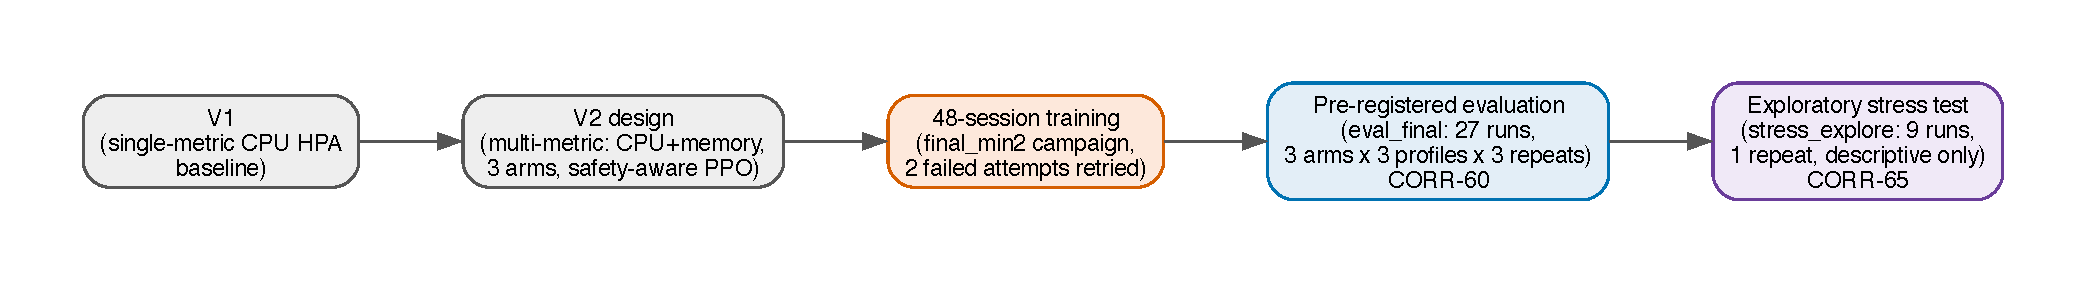
\includegraphics[width=0.9\textwidth]{../figures/diagram_experiment_pipeline.pdf}
\caption{The project's experiment pipeline: V1 design and evaluation,
leading to the V2 redesign, the 48-session V2 training campaign, the
pre-registered evaluation (\texttt{eval\_\allowbreak final}, CORR-60), and the later,
separately labelled exploratory stress test (\texttt{stress\_\allowbreak explore},
CORR-65), which never supersedes the pre-registered evaluation.}
\label{fig:experiment-pipeline}
\end{figure}

\section{Testbed}

We ran every experiment on a single-node Minikube cluster using the Docker
driver, on a MacBook Air with an Apple M1 chip and 8~GB of RAM, with Docker
Desktop providing the container runtime Minikube uses. We allocated 2 CPUs
and 3~GB of RAM to the Minikube virtual node. We chose a local, single-node
cluster over a cloud-hosted or multi-node cluster for a combination of
reasons specific to a capstone project's circumstances rather than any claim
that this is the right choice for production evaluation: it is free, it
gives us full, low-level visibility into node-level CPU and memory pressure
that a managed cluster would partly hide behind another layer of
virtualization, and it let us run both generations' full training and
evaluation campaigns, totalling tens of thousands of real decision steps,
without incurring cloud compute cost or depending on network conditions
outside our control. The obvious limitation of this choice, which we state
plainly in Section~\ref{sec:limitations}, is that a single-node cluster on a
laptop is not a multi-node production cluster, and some findings here (in
particular absolute resource headroom) may not transfer directly.

\section{Benchmark Service}

The benchmark service, in \texttt{app/\allowbreak \allowbreak }, is a small FastAPI application
exposing three endpoints: \texttt{/\allowbreak \allowbreak work}, \texttt{/\allowbreak \allowbreak health}, and
\texttt{/\allowbreak \allowbreak metrics}. The \texttt{/\allowbreak \allowbreak work} endpoint is the one all traffic
profiles target, and it supports two load modes, CPU and memory, selected
per request so that a traffic profile can be built out of a mix of both.
In CPU mode, the handler performs a bounded amount of synchronous
computation sized to hold the request for a target duration, which is what
lets our CPU-oriented traffic profiles push a pod's CPU usage up in a
controlled, repeatable way. In memory mode, the handler allocates and holds
a block of memory for the duration of the request, which is what lets our
memory-oriented profiles (\texttt{eval\_\allowbreak memory\_\allowbreak ramp},
\texttt{stress\_\allowbreak memory\_\allowbreak ramp}) exercise the memory side of the reward and
observation space rather than only CPU. \texttt{/\allowbreak \allowbreak health} is a liveness and
readiness endpoint used by Kubernetes probes; \texttt{/\allowbreak \allowbreak metrics} exposes
Prometheus-format counters and histograms, including request totals by
route, 5xx error totals, request latency, and the number of requests
currently in progress. Each pod is deployed with a CPU request of 100
millicores and a memory request of 64~MiB, with limits of 500 millicores
and 256~MiB; these specific values set the denominators used throughout the
observation space's per-replica ratio features (Section~\ref{sec:mdp}).

\section{Traffic Generator}

The traffic generator, in \texttt{loadgen/\allowbreak \allowbreak }, is open-loop and
deterministic: given a traffic profile and a seed, it produces exactly the
same schedule of requests every time it is replayed, which is what makes a
training session or an evaluation episode reproducible rather than subject
to whatever load the generator happened to produce that run. Being
open-loop means the generator issues requests on its own schedule and does
not slow down or speed up based on how the server is responding, which
mirrors how most real internet traffic behaves and avoids the generator
itself becoming an implicit extra feedback controller that could mask or
distort the autoscaler's own behaviour.

Traffic profiles are organized into four disjoint sets, each firewalled
from the others by an explicit allowlist in the training and evaluation
code so that a profile used for one purpose can never silently leak into
another: a \textbf{training} set used only during the PPO training campaign
(constant CPU, constant memory, constant mixed, mixed ramp, and mixed burst
profiles, cycled through a seeded shuffle); an \textbf{evaluation} set used
only for the pre-registered \texttt{eval\_\allowbreak final} campaign
(\texttt{eval\_\allowbreak cpu\_\allowbreak step}, \texttt{eval\_\allowbreak memory\_\allowbreak ramp},
\texttt{eval\_\allowbreak mixed\_\allowbreak burst}, each peaking at 18-20 requests per second, well
below training-level peaks); a \textbf{stress} set used only for the later,
exploratory \texttt{stress\_\allowbreak explore} campaign (\texttt{stress\_\allowbreak cpu\_\allowbreak burst},
\texttt{stress\_\allowbreak memory\_\allowbreak ramp}, \texttt{stress\_\allowbreak mixed\_\allowbreak burst}, peaking at
45-70 requests per second, at the same peaks already exercised live during
training, never beyond); and a \textbf{demo} set used only by the Streamlit
demonstration console. Table~\ref{tab:eval-profiles} in
Section~\ref{sec:eval-protocol} gives the exact peak rate and resource mode
of each evaluation and stress profile. This firewall exists because the
whole point of an evaluation is to test a controller on traffic it has not
seen; if a profile used in training could also appear in evaluation, even
accidentally, any advantage shown there would be unfalsifiable.

\section{Telemetry and PromQL Signals}

Every signal the RL agent's observation builder uses, and every signal our
evaluation analysis computes, comes from Prometheus, not from the Metrics
Server (the HPA baselines read the Metrics Server for CPU/memory directly,
through the Kubernetes Horizontal Pod Autoscaler controller's own internal
path, which we do not reimplement). The raw metrics read from Prometheus
are: \texttt{demo\_\allowbreak app\_\allowbreak requests\_\allowbreak total} (counter, by route, used via
\texttt{rate()} over a window to get request rate), 5xx error totals (used
the same way to get error rate -- live-observable reliability in this
project is 5xx-only; client-side timeouts and connection errors are not
available to a live policy and are only ever used in offline analysis),
a request latency histogram (used to compute a 95th-percentile, p95,
latency estimate), \texttt{demo\_\allowbreak app\_\allowbreak requests\_\allowbreak in\_\allowbreak progress} (gauge),
container CPU core usage and memory byte usage per pod (from
\texttt{cadvisor}-derived metrics scraped by Prometheus), and the
Deployment's ready and current replica counts, read from the Kubernetes API
rather than Prometheus. We verified the Metrics Server's own resolution at
15 seconds live, immediately before every HPA-arm run, rather than assuming
it; we also verified before every HPA run that Prometheus and the Metrics
Server were both healthy, since both the RL agent and every HPA arm depend
on telemetry being available.

\section{MDP Formulation}
\label{sec:mdp}

We formalize the autoscaling problem as a Markov Decision Process with a
30-second decision interval. At each decision point the agent observes an
eleven-feature vector derived from the raw telemetry above, chooses one of
three actions, and that action -- after passing through the deterministic
safety layer of Section~\ref{sec:safety-layer} -- is applied to the
Deployment's replica count. Thirty seconds later the cycle repeats. One
episode is one full playback of a traffic profile.

\subsection{Observation Features}

Table~\ref{tab:observation-features} gives the eleven observation features
in the exact order the policy network sees them, their raw ranges, how they
are normalized into $[-1,1]$ or $[0,1]$ before being passed to the network,
and whether each is an instantaneous ("current") feature or a trend
feature. Index 0-8 are clipped to their stated raw range and then divided by
that range's width; index 9 (ready replicas) is normalized against the
V2 replica floor and ceiling (2 and 8); index 10 (seconds since the last
effective scaling action) is clipped at a 300-second cap and divided by
that cap. The four trend features (indices 1, 5, 7, and implicitly the
EWMA state behind them) are each the current step's value minus a
90-second exponentially weighted moving average of that same signal, so
that the agent can distinguish "CPU is high and rising" from "CPU is high
and falling" using the same instantaneous value.

\begin{table}[H]
\centering
\caption{The eleven V2 observation features, in network input order.}
\label{tab:observation-features}
\small
\begin{tabular}{p{0.6cm}p{2.6cm}p{6.2cm}p{1.6cm}p{1.7cm}p{1.3cm}}
\hline
index & name & meaning & raw\_range & normalized\_range & temporal \\
\hline
0 & cpu\_per\_replica & (cpu\_cores / ready\_replicas) / 0.100, i.e. fraction of the 100m CPU request per Ready replica -- a NOMINALLY COMPARABLE proxy to HPA's averageUtilization/100, not literally identical to it (docs/rl\_mdp\_spec.md sec.4, CORR-27). & [0.0, 5.0] & [0.0, 1.0] & current \\
1 & cpu\_per\_replica\_delta & current step's cpu\_per\_replica minus its 90s EWMA (momentum/trend, not a raw one-step difference). & [-5.0, 5.0] & [-1.0, 1.0] & trend \\
2 & memory\_per\_replica & (memory\_bytes / ready\_replicas) / 67108864, i.e. fraction of the 64MiB memory request per Ready replica. & [0.0, 4.0] & [0.0, 1.0] & current \\
3 & in\_progress\_per\_replica & requests\_in\_progress / ready\_replicas -- secondary queueing-pressure signal, redundant with CPU on this CPU-bound app but retained per Phase 15A evaluation for robustness. & [0.0, 20.0] & [0.0, 1.0] & current \\
4 & request\_rate\_norm & sum(\allowbreak rate(\allowbreak demo\_app\_requests\_total\allowbreak \{route="/work"\}[1m])), normalized against a 100 RPS design ceiling, justified ONLY from non-held-out development profile peaks (burst=70, ramp=60, step=50 RPS). Never justified from any held-out evaluation workload's parameters (CORR-27; see docs/rl\_mdp\_spec.md sec.22). & [0.0, 100.0] & [0.0, 1.0] & current \\
5 & request\_rate\_delta & current step's request\_rate\_rps minus its 90s EWMA. & [-100.0, 100.0] & [-1.0, 1.0] & trend \\
6 & p95\_latency\_norm & latency\_p95\_seconds (ms), normalized against a 2000ms ceiling (~6.67x the 300ms SLA target). If request\_rate\_rps==0 with no histogram observations, this is semantically 0ms ("no\_traffic", CORR-27) -- not a telemetry failure; see docs/rl\_mdp\_spec.md sec.6. & [0.0, 2000.0] & [0.0, 1.0] & current \\
7 & p95\_latency\_delta & current step's p95 latency (ms) minus its 90s EWMA. & [-2000.0, 2000.0] & [-1.0, 1.0] & trend \\
8 & error\_rate & error\_rate\_rps (5xx only, live-observable) / request\_rate\_rps; 0.0 if request\_rate\_rps==0; null (missing) if request\_rate\_rps is null. & [0.0, 1.0] & [0.0, 1.0] & current \\
9 & ready\_replica\_norm & (replicas\_ready - 2) / (8 - 2) -- authoritative physical capacity, never hpa\_status\_current\_replicas (CORR-25). Normalized against a replica floor of 2 and ceiling of 8 (CORR-55); the floor is 2, never 1. & [2.0, 8.0] & [0.0, 1.0] & current \\
10 & seconds\_since\_last\_scale\_norm & controller-tracked seconds since the last EFFECTIVE (non-HOLD) action, capped per experiment.yaml rl.time\_since\_scale\_cap\_seconds. & [0.0, 300.0] & [0.0, 1.0] & current \\
\hline
\end{tabular}

\end{table}

\subsection{Normalization and Missing-Data Rules}
\label{sec:invalid-telemetry}

Two distinct situations have to be told apart carefully, and conflating
them was a source of an early V1-era bug (CORR-56) that we describe in
Section~\ref{sec:v1-to-v2}: genuine zero traffic, and missing or unreliable
telemetry. When the request rate is genuinely zero and no latency
histogram observations exist for the window, the p95 latency feature is
defined as exactly 0~ms -- this is a valid, meaningful state ("no traffic
right now"), not a sign that something is wrong, and it participates
normally in the EWMA trend calculation. When the request rate is nonzero
but a usable latency estimate cannot be computed, or any other required raw
signal cannot be read for the window, the sample is marked invalid; on an
invalid sample, every level and trend feature except the two
controller-tracked ones (ready-replica count and seconds-since-last-scale,
both of which come from state the controller itself always knows,
independent of Prometheus) holds its previous normalized value rather than
being set to zero, the clip maximum, or any other fabricated number. The
very first decision of an episode, before any previous value exists, uses
the raw-range midpoint for every held feature and is flagged as such. Four
consecutive invalid decisions (two minutes of persistently unusable
telemetry at the 30-second interval) terminate the episode; one to three
consecutive invalid decisions instead force a deterministic HOLD action for
that step, through the same safety layer that governs every other case
requiring a fallback.

\section{Action Space and Safety Layer}
\label{sec:safety-layer}

The action space is \texttt{Discrete(3)}: remove one replica
(\textsc{scale\_down\_one}), hold the current replica count
(\textsc{hold}), or add one replica (\textsc{scale\_up\_one}). The policy
network never outputs a replica count directly and never outputs a
multi-replica jump; every decision changes the Deployment by at most one
replica, which keeps the action space small and keeps every single action's
effect easy to reason about and to log.

Between the policy's raw action and the Kubernetes API sits a deterministic
safety layer that the learned policy cannot see into or override. Its rules
are, in the order they are checked: a replica-bound clamp, so that a
requested delta that would take the Deployment below the configured floor
or above the configured ceiling is converted to a no-op with that clamp
recorded as the override reason; a pending-scale gate, so that if the
Deployment's desired and ready replica counts currently disagree (a scaling
action is already in flight), any further non-hold action is overridden to
hold until the pending change settles; and an asymmetric cooldown, so that
a scale-up action is never delayed by this gate beyond ordinary pending-scale
settling, while a scale-down action additionally requires at least 60
seconds to have passed since the last effective scaling action of any
direction. This asymmetry is deliberate: it lets the controller react to a
sudden spike immediately, in either generation's design, while making
scaling down a more deliberate, slower action that cannot immediately
reverse an upward move -- the asymmetric cooldown further explicitly allows
an "emergency reversal" (an immediate scale-up right after a scale-down) to
pass through ungated, since erring toward more capacity is never penalized
by this gate. Listing~\ref{lst:gating} in Appendix~\ref{ch:appendix} gives
the gating function in full.

\subsection{Safety-Aware Tie-Breaking}
\label{sec:tie-break}

A separate concern from gating is what the controller should do when the
policy's own output does not clearly favour one action. For deterministic
evaluation, Stable-Baselines3's default behaviour is to take the
arg-max of the policy's action probabilities; when two or more actions are
within a small margin of each other, an arg-max breaks the tie toward the
lowest action index, which in our action encoding is
\textsc{scale\_down\_one} -- meaning an uncertain policy would be silently
biased toward removing capacity purely as an artefact of how ties are
broken, never because removing capacity was actually the better action
on the merits. We replaced this default with a safety-aware tie-break rule
(CORR-58), used only for deterministic inference during evaluation, never
during training (Stable-Baselines3's own stochastic sampling during
\texttt{model.learn()} never passes through this code path). The rule
first computes the tie set: every action whose probability is within
$\varepsilon$ of the maximum probability. If the tie set has exactly one
member, that action is chosen (rule R1) and the controller's own inference
log records this as "no tie," which is what happens on the overwhelming
majority of decisions. If the tie set is larger than one, the following
rules apply, in order, and are illustrated in
Figure~\ref{fig:tie-break-flow}:

\begin{itemize}[nosep]
  \item \textbf{R2}: \textsc{scale\_down\_one} can never, by construction,
    be the output of a tie -- it structurally never wins when tied with
    anything else.
  \item \textbf{R3}: a tie between \textsc{hold} and
    \textsc{scale\_up\_one} resolves to \textsc{scale\_up\_one} if the
    system is currently judged \emph{stressed}, and to \textsc{hold}
    otherwise.
  \item \textbf{R4}: a tie between \textsc{scale\_down\_one} and
    \textsc{scale\_up\_one}, or a three-way tie among all actions, resolves
    to \textsc{hold}.
  \item \textbf{R5}: a tie between \textsc{scale\_down\_one} and
    \textsc{hold} resolves to \textsc{hold}.
  \item \textbf{R6}: if whether the system is stressed cannot be determined
    (for example, because the raw observation needed to judge it is itself
    missing), the rule fails safe to \textsc{hold}.
\end{itemize}

\begin{figure}[htbp]
\centering
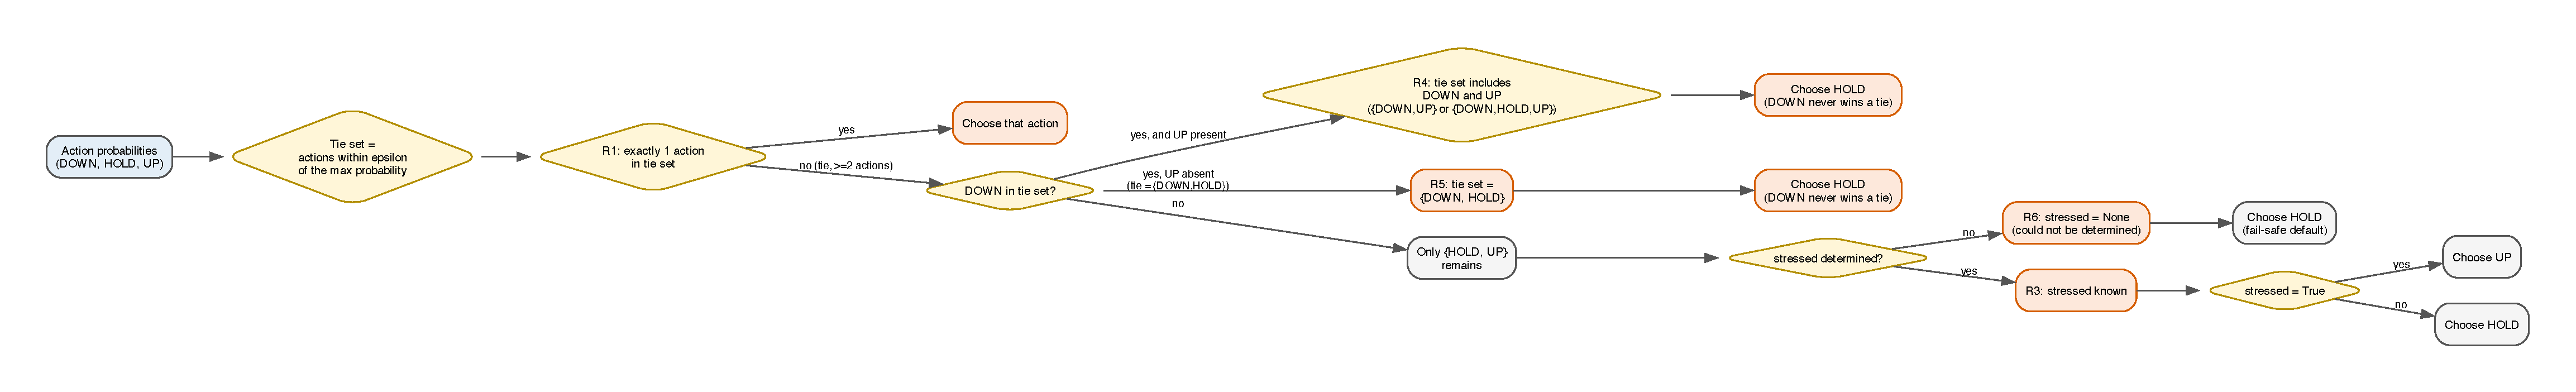
\includegraphics[width=0.78\textwidth]{../figures/diagram_tie_break_flow.pdf}
\caption{Decision flow for the safety-aware tie-break rule (R1-R6,
CORR-58): from the PPO action-probability tie set to the final selected
action. \textsc{scale\_down\_one} can never win a tie by construction; an
unknown-stress tie fails safe to \textsc{hold}.}
\label{fig:tie-break-flow}
\end{figure}

"Stressed" is defined from the same decision-time raw observation the
policy itself sees: the system is stressed if p95 latency is at or above
the SLA target, or the error rate is above zero, or CPU or memory per ready
replica is above its configured "safe-high" threshold (the same thresholds
used in the V2 pressure reward term, Section~\ref{sec:v2-reward}). The
intent, stated in our own design-correction log, is availability-first
behaviour under genuine stress -- scale up quickly when the signals say the
system is actually under load, roughly mirroring how a conventional HPA
would react -- while never letting scale-down be the accidental outcome of
an uncertain policy rather than a deliberate one.

\subsection{Epsilon Calibration}

The tie-break margin $\varepsilon$ was calibrated, not guessed, and
calibrated before the pre-registered evaluation it would be used in, not
after. We computed the margin between each decision's top and second
probability over the final training checkpoint's behaviour on the last
five training sessions (sessions 43-47), took the 10th percentile of that
margin distribution, and capped the result at 0.05 (floored at 0.0). The
raw 10th-percentile value came out above the cap, so the calibrated
$\varepsilon$ used throughout evaluation is 0.05. Only 0.55\% of decisions
in that calibration window fell inside a tie at this value, and in the
actual pre-registered evaluation, the tie-break rule changed the outcome of
only 4 of 360 PPO decisions (1.11\%; Figure~\ref{fig:tie-rule-frequency} in
Chapter~\ref{ch:results}) -- the safety-aware rule is a rare, deliberately
narrow intervention, not a mechanism that drives most decisions.

\section{V1 Reward Function}
\label{sec:v1-reward}

V1's reward combined a latency penalty, an error penalty, an unconditional
per-replica resource cost, small action/reversal/boundary penalties, and a
positive "efficiency" bonus. In the exact form frozen for V1
(\texttt{docs/\allowbreak \allowbreak rl\_\allowbreak mdp\_\allowbreak spec.md}, \texttt{rl\_\allowbreak contract\_\allowbreak version 2},
CORR-27):
\begin{equation}
r_t = -\min(e_t^2, 4) - 5\rho_t - \frac{n_t-1}{7} - 0.1\,\mathbb{1}_{\text{act}} - 0.5\,\mathbb{1}_{\text{rev}} - 0.2\,\mathbb{1}_{\text{bnd}} + 0.3\,\mathbb{1}_{\text{eff}}
\label{eq:v1-reward}
\end{equation}
where $e_t = \max(0, p_t - 300)/300$ is the fractional excess of p95 latency
$p_t$ (in milliseconds) above a 300~ms target, $\rho_t$ is the 5xx error
fraction, $n_t$ is the current replica count (so the resource term grows
toward 1 as replicas approach the 8-replica ceiling and is paid on
\emph{every} step regardless of whether the extra replicas are doing any
good), and the indicator terms penalize taking any non-hold action, any
direction reversal within a window, and any action clamped at a replica
bound; the efficiency bonus rewards a step where CPU per replica sits
between $1.0\times$ and $3.0\times$ the CPU request, latency is below
target, and there are no errors. The critical property of
Equation~\ref{eq:v1-reward} for what follows is the unconditional resource
term $-(n_t-1)/7$: it charges a cost for every replica above one,
\emph{every single step}, whether or not the system actually needed those
replicas, and it does so regardless of the pod health that produced that
replica count.

\section{PPO Algorithm and Hyperparameters}

Both generations used the same PPO implementation (Stable-Baselines3
\cite{raffin2021sb3}) and the same core hyperparameters, summarized in
Table~\ref{tab:ppo-hyperparams}, with a two-layer, 128-unit multilayer
perceptron for both the policy and value networks, no hyperparameter
search performed, and a fixed training seed (42) throughout. One detail
specific to this project's live-cluster setting is the rollout length: PPO
defaults in Stable-Baselines3 to collecting 2048 steps between updates,
which at a 30-second decision interval would mean roughly 17 hours between
updates; we instead collect 256 steps (one "session") between updates, so
that each training session completes in a practical wall-clock time and
checkpoints at a useful cadence, at the cost of each PPO update seeing a
smaller batch of fresh experience than the library's own default assumes.

\begin{table}[H]
\centering
\caption{PPO hyperparameters used for both V1 and V2 training.}
\label{tab:ppo-hyperparams}
\begin{tabular}{ll}
\hline
parameter & value \\
\hline
learning\_rate & 0.0003 \\
n\_steps & 2048 \\
batch\_size & 64 \\
n\_epochs & 10 \\
gamma & 0.99 \\
gae\_lambda & 0.95 \\
clip\_range & 0.2 \\
ent\_coef & 0.01 \\
vf\_coef & 0.5 \\
max\_grad\_norm & 0.5 \\
policy & MlpPolicy \\
net\_arch & [128, 128] \\
training\_budget & 48 sessions x 256 steps/session = 12288 total timesteps (final\_min2 campaign) \\
\hline
\end{tabular}

\end{table}

\section{Session, Checkpoint, and Resume Design}

Training proceeds in sessions of 256 decision steps each; every session
ends with a Stable-Baselines3 checkpoint (\texttt{ppo\_\allowbreak model.zip}), the
environment's own random-number-generator state (so a resumed session
reproduces the same stochastic choices it would have made had it not
stopped), and session metadata recording cumulative timesteps, cumulative
PPO updates, and which sessions have completed. A campaign can be resumed
from its last completed session rather than restarted from scratch, which
matters in practice: of the V2 campaign's 48 planned sessions, two
(sessions 4 and 38) failed partway through and had to be resumed from the
last good checkpoint rather than from session zero, a design choice that
turned a potential multi-day restart into a same-day recovery. We discuss
both failures, and what caused them, in Chapter~\ref{ch:results}.

\section{Freeze Manifest, Correction Log, and Pre-Registration}

Three documents together are this project's reproducibility methodology,
and we treat them as load-bearing rather than as paperwork. The
\textbf{freeze manifest} (\texttt{FREEZE\_\allowbreak MANIFEST.json}, with two later
amendments) records SHA-256 hashes of every file governing a training
campaign -- the environment code, the reward implementation, the
configuration files, the PPO hyperparameters, the live cluster's resource
limits at freeze time -- at the moment the final V2 campaign began; any
post-freeze change to a hashed file invalidates that campaign's checkpoints
for resumption, verified automatically rather than trusted to memory. The
\textbf{correction log} (\texttt{docs/\allowbreak \allowbreak experimental\_\allowbreak design\_\allowbreak corrections.md})
is an append-only record of every design decision and mid-course
correction made across the whole project, numbered CORR-1 through CORR-65,
each with its problem, decision, scope, scientific impact, and
non-retroactivity explicitly stated; nothing in this project is corrected
silently, and a reader can always find out exactly when and why a given
rule changed. The \textbf{pre-registration}
(\texttt{docs/\allowbreak \allowbreak evaluation\_\allowbreak v2\_\allowbreak preregistration.md}, CORR-60) fixes the
evaluation's arms, traffic profiles, metrics, retry rules, and decision
rule in writing before any V2 evaluation episode ran -- before the final
training checkpoint (session 47) even existed. We refer back to specific
CORR entries throughout this chapter and the next, both because they are
the authoritative source for each design decision and because a reader
who wants the full detail behind a short summary here can look it up by
number; Appendix~\ref{ch:appendix} gives a complete table of every CORR
entry.

\section{V1 to V2 Redesign}
\label{sec:v1-to-v2}

V1's evaluation (Chapter~\ref{ch:results}) did not produce a usable
PPO-versus-HPA verdict: of three required valid PPO repeats, only one
completed without a safety termination. Diagnosing why led to the V2
redesign summarized in Table~\ref{tab:v1-v2-comparison}; none of these
changes were made casually, and each is backed by a numbered correction in
the log.

\begin{table}[H]
\centering
\caption{Design differences between V1 and V2, and the reason for each.}
\label{tab:v1-v2-comparison}
\small
\begin{tabular}{p{2.6cm}p{2.9cm}p{2.9cm}p{4.3cm}}
\toprule
Aspect & V1 & V2 & Reason for the change \\
\midrule
Observation signals & CPU-derived only (1 primary dimension) & 11 features: CPU, memory, request rate, latency, replica state, all 4 with short-horizon trends & A CPU-only view cannot represent memory-bound load or anticipate a trend; V2's benchmark service and traffic profiles deliberately exercise memory as well as CPU. \\
Replica floor & 1 & 2 (CORR-55) & Both live V1-era attempts at scientific session index 3 of V2 final training failed with the Deployment's entire ready-replica count driven to zero by a single pod's own saturation or restart -- a floor of 1 gives the whole system no redundancy against one pod's transient unhealthiness. \\
Resource/waste cost & Unconditional, every step, proportional to replica count & Conditional "waste" penalty, fires only when replicas exceed the floor \emph{and} CPU/memory are both low \emph{and} latency/error are already healthy & V1's unconditional cost made adding a replica look bad even when the system genuinely needed it, biasing the policy toward staying small regardless of actual load. \\
SLA target (p95) & 300\,ms & 1000\,ms (CORR-57) & Memory-mode requests legitimately hold for close to 500\,ms; combined with Prometheus histogram-bucket interpolation, this was being reported near 975\,ms and permanently penalized against a 300\,ms target that the workload could not realistically meet. \\
Deterministic tie-break & SB3 default arg-max (ties toward lowest action index, i.e.\ scale-down) & Safety-aware rule, scale-down can never win a tie (CORR-58) & An uncertain policy should never have its uncertainty silently resolved toward removing capacity. \\
Comparison baseline(s) & One tuned HPA (CPU only) & Two HPA arms: CPU+memory (resource baseline) and CPU-only (CPU baseline), both at the V2 floor of 2 (CORR-62) & Isolates whether the memory metric matters and whether the higher replica floor alone explains any difference, rather than conflating both changes in a single baseline. \\
Training budget & 5,120 timesteps (20 sessions), cut short by live-cluster wall-clock constraints & 12,288 timesteps (48 sessions), amended and recorded before any post-amendment session result existed (CORR-59) & V1's budget was not a deliberate scientific choice; V2's budget change was decided and logged while only session 0 had been reviewed, avoiding an outcome-aware budget increase. \\
\bottomrule
\end{tabular}
\end{table}

\section{V2 Reward Function}
\label{sec:v2-reward}

The V2 reward replaces V1's unconditional resource cost and latency-only
penalty with seven components, each independently weighted, summarized in
Table~\ref{tab:reward-components} and defined in full in
\texttt{configs/\allowbreak \allowbreak reward\_\allowbreak v2.yaml} (Listing~\ref{lst:reward-config} in
Appendix~\ref{ch:appendix}):
\begin{equation}
r_t = -\big(w_{\text{rel}}\rho_t + w_{\text{sla}}\,\mathrm{sla}_t + w_{\text{prs}}\,\mathrm{prs}_t + w_{\text{wst}}\,\mathbb{1}_{\text{waste}} + w_{\text{act}}\,\mathbb{1}_{\text{act}} + w_{\text{rev}}\,\mathbb{1}_{\text{rev}} + w_{\text{bnd}}\,\mathbb{1}_{\text{bnd}}\big)
\label{eq:v2-reward}
\end{equation}
with $\rho_t$ the clipped 5xx error fraction; $\mathrm{sla}_t =
\mathrm{clip}(e_t^2, 0, 1)$ the clipped squared excess of p95 latency above
the 1000~ms target, $e_t = \max(0, p_t-1000)/1000$; and
$\mathrm{prs}_t = \max(\mathrm{prs}_{\text{cpu}}, \mathrm{prs}_{\text{mem}})$
the worse of a CPU and a memory "pressure" term, each defined as the
clipped, squared fraction of the way a per-replica utilization has moved
from a "safe-high" threshold toward a hard resource limit:
$\mathrm{prs}_{\text{cpu}} = \mathrm{clip}\!\left(\frac{u_{\text{cpu}} -
3.0}{5.0-3.0}, 0, 1\right)^2$ and similarly for memory with thresholds
1.2 and 4.0. The waste indicator fires only when the current replica count
is above the floor \emph{and} CPU and memory per replica are both below
their waste thresholds \emph{and} latency and error are already healthy --
by construction, a policy cannot lower its waste cost by staying small
while the system is in genuine distress, because the waste term simply does
not apply in that state. Action, reversal, and boundary penalties are
unchanged in shape from V1.

\begin{table}[H]
\centering
\caption{V2 reward components, weights, and threshold parameters.}
\label{tab:reward-components}
\small
\begin{tabular}{p{2cm}p{1cm}p{7.2cm}p{4.3cm}}
\hline
component & weight & meaning & threshold\_params \\
\hline
w\_reliability & 6.0 & Penalizes the live 5xx error rate (clipped to [0,1]). & n/a \\
w\_sla & 4.0 & Penalizes squared excess p95 latency above the SLA target (clipped to [0,1]). & p95\_target\_ms=1000 \\
w\_pressure & 2.0 & Penalizes the worse of CPU/memory 'unsafe pressure' (distance toward the pod's hard resource limit). & cpu\_safe\_high=3.0, cpu\_hard\_limit=5.0, memory\_safe\_high=1.2, memory\_hard\_limit=4.0 \\
w\_waste & 0.3 & Penalizes over-provisioning (replicas > floor, low CPU+memory, SLA/error already healthy). & cpu\_waste\_threshold=1.0, memory\_waste\_threshold=1.0 \\
w\_action & 0.1 & Penalizes taking any non-HOLD action (discourages unnecessary churn). & per\_action\_cost=1.0 \\
w\_reversal & 0.5 & Penalizes reversing a scaling direction within the reversal window (discourages oscillation). & reversal\_window\_seconds=120, per\_reversal\_cost=1.0 \\
w\_boundary & 0.2 & Penalizes an action clamped at the replica floor/ceiling (discourages pushing against the bound). & per\_boundary\_violation\_cost=1.0 \\
\hline
\end{tabular}

\end{table}

\section{Evaluation Protocol}
\label{sec:eval-protocol}

\subsection{Arms and Profiles}

Table~\ref{tab:eval-arms} lists the three arms compared in both the
pre-registered evaluation and the exploratory stress test; all three use
identical replica bounds (2-8) and the identical benchmark application
image, so that the only thing that differs between arms is the controller
itself. Table~\ref{tab:eval-profiles} lists the traffic profiles each
campaign uses.

\begin{table}[H]
\centering
\caption{Evaluation arms.}
\label{tab:eval-arms}
\resizebox{\linewidth}{!}{\begin{tabular}{lll}
\hline
arm & profiles\_run\_on & role \\
\hline
PPO (multi-metric, 11 signals) & all 3 held-out + all 3 stress & RL policy under test \\
HPA CPU+Memory & all 3 held-out + all 3 stress & resource-metric baseline (CPU and memory, 260\%/120\% targets) \\
HPA CPU-only (CPU baseline) & all 3 held-out + all 3 stress & single-metric baseline (CPU only, same 260\% target and 2-8 bounds as the others) \\
\hline
\end{tabular}
}
\end{table}

\begin{table}[H]
\centering
\caption{Traffic profiles used by the pre-registered evaluation
(\texttt{eval\_\allowbreak final}) and the exploratory stress test
(\texttt{stress\_\allowbreak explore}).}
\label{tab:eval-profiles}
\resizebox{\linewidth}{!}{\begin{tabular}{lllll}
\hline
campaign & profile & resource\_mode & peak\_rps & repeats \\
\hline
eval\_final (pre-registered, CORR-60) & eval\_cpu\_step & cpu & 18.0 & 3 \\
eval\_final (pre-registered, CORR-60) & eval\_memory\_ramp & memory & 18.0 & 3 \\
eval\_final (pre-registered, CORR-60) & eval\_mixed\_burst & mixed & 20.0 & 3 \\
stress\_explore (exploratory, CORR-65) & stress\_cpu\_burst & cpu & 70.0 & 1 \\
stress\_explore (exploratory, CORR-65) & stress\_memory\_ramp & memory & 45.0 & 1 \\
stress\_explore (exploratory, CORR-65) & stress\_mixed\_burst & mixed & 70.0 & 1 \\
\hline
\end{tabular}
}
\end{table}

\subsection{Design and Order}

The pre-registered \texttt{eval\_\allowbreak final} campaign ran 3 repeats of every
(profile, arm) cell: 3 profiles $\times$ 3 arms $\times$ 3 repeats = 27
planned runs. The order of the three arms within each repeat was rotated
using a Latin square, so that no arm was systematically run first or last
within a repeat -- a precaution against any systematic drift in cluster
state (for example, residual caching or thermal effects) that could
otherwise confound arm identity with run order. Before every HPA-arm run we
verified Metrics Server resolution and cluster health live rather than
assuming them, and Grafana was scaled to zero replicas for the whole V2
evaluation campaign so that it could not compete with the benchmark
application for the Minikube node's limited CPU and memory, and so that it
could not itself add any confounding load to the cluster during a
measured run.

\subsection{Metrics and Decision Rule}

The primary metrics, fixed in the pre-registration before any evaluation
run, are SLA-violation rate at the 1000~ms target and replica-minutes (the
time-integral of replica count, our cost proxy). Secondary metrics include
mean and median p95 latency, error rate, maximum per-pod memory, scaling
action count, reversal count, pod restart count, invalid-sample count, and
an SLA-violation rate at a 300~ms reference threshold kept only for
historical comparability with V1. Table~\ref{tab:decision-rule} states the
decision rule exactly as pre-registered: an arm is only reported as
"better" than another on a given metric for a given profile if it is
better in all three of the three repeats, and no single aggregate winner is
declared when different metrics disagree -- such cases are reported
explicitly as a trade-off rather than resolved into one ranking.

\begin{table}[H]
\centering
\caption{Pre-registered decision rule (CORR-60).}
\label{tab:decision-rule}
\small
\begin{tabular}{p{3cm}p{12cm}}
\hline
rule & statement \\
\hline
reporting & Per profile, per arm: report mean +/- standard deviation over the 3 repeats for every metric. \\
claiming\_better & An arm may be claimed 'better' than another on a given metric for a given profile ONLY if it is better in ALL 3 of the 3 repeats (not merely on average) -- a single repeat going the other way blocks the claim for that metric/profile pair. \\
no\_aggregate\_winner & No single aggregate 'winner' is declared across metrics that disagree (e.g. one arm has a lower SLA-violation rate but higher replica-minutes) -- such cases are reported explicitly as a trade-off, not resolved into a single ranking. \\
applies\_to & eval\_final only (3 repeats/cell). Does NOT apply to stress\_explore (1 repeat/cell, descriptive only, CORR-65). \\
\hline
\end{tabular}

\end{table}

\subsection{Retry Rules}

A tooling failure -- an unreachable route, a down Prometheus instance, a
cluster or network fault, none of which reflects anything about either
controller's scaling behaviour -- results in no scientific outcome being
recorded for that attempt and exactly one retry; the failed attempt's
evidence is preserved, never deleted. A safety termination (a sustained
loss of ready replicas, or a memory threshold breach) is, by contrast,
counted as a real scientific outcome of that run and is never retried,
because a safety termination is itself a fact about how the controller
behaved under that traffic, not a tooling artefact to be papered over.

\section{The Demo UI}

\texttt{demo\_\allowbreak ui/\allowbreak \allowbreak } is a Streamlit console used to inspect training curves,
replay evaluation episodes, and view live cluster state during
development and demonstration. It runs in a demo/fixture mode by default
and does not require a live cluster to start, falling back to cached or
fixture data when a live connection is unavailable, so that it can be used
for a demonstration without first standing up the full testbed. It reads
the same \texttt{persistent-data/\allowbreak \allowbreak } artifacts (training session metadata,
evaluation run ledgers) that the analysis scripts in
Section~\ref{sec:software-stack} read, rather than maintaining its own
separate copy of this data, so that what the UI shows and what the
published figures and tables show cannot drift apart.

\section{Software Stack and Hardware}
\label{sec:software-stack}

Table~\ref{tab:software-stack} lists the key software dependencies and the
exact versions pinned in the project's requirements files.
Table~\ref{tab:hardware} lists the hardware used for every training and
evaluation run reported in this document.

\begin{table}[H]
\centering
\caption{Key software dependencies and pinned versions.}
\label{tab:software-stack}
\begin{tabular}{ll}
\toprule
Component & Version \\
\midrule
Python & 3.10.14 \\
Kubernetes Python client & 31.0.0 \\
FastAPI & 0.115.6 \\
Uvicorn & 0.32.1 \\
Prometheus client (Python) & 0.21.1 \\
prometheus-api-client & 0.5.5 \\
NumPy & 1.26.4 \\
Pandas & 2.2.3 \\
Stable-Baselines3 & 2.6.0 \\
Gymnasium & 1.1.1 \\
PyTorch & 2.5.1 \\
Matplotlib & 3.10.9 \\
scikit-learn & 1.6.1 \\
Streamlit (demo UI) & 1.65.0 \\
Plotly (demo UI) & 7.1.0 \\
\bottomrule
\end{tabular}
\end{table}

\begin{table}[H]
\centering
\caption{Hardware used for all training and evaluation runs.}
\label{tab:hardware}
\begin{tabular}{ll}
\toprule
Item & Specification \\
\midrule
Host laptop & MacBook Air, Apple M1, 8\,GB RAM \\
Container runtime & Docker Desktop \\
Kubernetes cluster & Minikube, single node, Docker driver \\
Cluster CPU allocation & 2 vCPU \\
Cluster memory allocation & 3\,GB \\
\bottomrule
\end{tabular}
\end{table}

\section{Integration and Workflow}

Putting the pieces together, a single evaluation attempt proceeds as
follows: the harness runs a preflight check (cluster, Prometheus, Metrics
Server health); it acquires the arm's controller identity under the
exclusivity lock, deleting any HPA object left behind by a previous arm so
that a stale controller cannot interfere; it starts the traffic generator
against the configured profile; the active controller (PPO or one of the
two HPA configurations) scales the Deployment for the length of the
episode; telemetry is recorded throughout; the generator is stopped and
drained; the cluster is cleaned up and settled back to canonical idle
state; and the attempt's full result, success or failure, is written to the
run's own directory and to the campaign's ledger. The same orchestration
code path, \texttt{scripts/\allowbreak \allowbreak evaluate\_\allowbreak v2\_\allowbreak campaign.py}, runs both the
pre-registered evaluation and the later exploratory stress test, differing
only in which traffic profiles and repeat counts are configured, which is
part of why we can state confidently that the two campaigns are run under
identical operational discipline even though their scientific status (a
decision-rule-bearing evaluation versus a descriptive, single-repeat
exploration) is very different.
